%%%%%%%%%%%%%%%%%%%%%%%%%%%%%%%%%%%%%%%%%%%%%%%%%%%%%%%%%%%%%%%%%%%%%%%%%%%%%%%%%%%%%%%%%%%%%%%%%%%%%%%%%%%
%                                           PACKAGES                                                      %
%%%%%%%%%%%%%%%%%%%%%%%%%%%%%%%%%%%%%%%%%%%%%%%%%%%%%%%%%%%%%%%%%%%%%%%%%%%%%%%%%%%%%%%%%%%%%%%%%%%%%%%%%%%
\documentclass[12pt, fleqn]{article}
\usepackage{amsmath, amsfonts, amsthm, amssymb, graphicx, enumitem, mathtools, MnSymbol, relsize, cancel}
\usepackage{siunitx}
\usepackage{pdfpages}
\usepackage{graphicx}
\usepackage[utf8]{inputenc}
\usepackage{biblatex}
\usepackage{pythontex}
\usepackage{listings}
\usepackage[pdftex,pdfpagelabels,bookmarks,hyperindex,hyperfigures]{hyperref}
\hypersetup{colorlinks=true,allcolors=blue}
\usepackage{hypcap}
\usepackage{float}
\usepackage{geometry}
\geometry{margin=1in}
%%%%%%%%%%%%%%%%%%%%%%%%%%%%%%%%%%%%%%%%%%%%%%%%%%%%%%%%%%%%%%%%%%%%%%%%%%%%%%%%%%%%%%%%%%%%%%%%%%%%%%%%%%%
%                                           REFERENCE FILE                                                %
%%%%%%%%%%%%%%%%%%%%%%%%%%%%%%%%%%%%%%%%%%%%%%%%%%%%%%%%%%%%%%%%%%%%%%%%%%%%%%%%%%%%%%%%%%%%%%%%%%%%%%%%%%%
\usepackage[export]{adjustbox}
\graphicspath{ {images/} }
%%%%%%%%%%%%%%%%%%%%%%%%%%%%%%%%%%%%%%%%%%%%%%%%%%%%%%%%%%%%%%%%%%%%%%%%%%%%%%%%%%%%%%%%%%%%%%%%%%%%%%%%%%%
%                                          PREPARE TITLE AND ABSTRACT                                     %
%%%%%%%%%%%%%%%%%%%%%%%%%%%%%%%%%%%%%%%%%%%%%%%%%%%%%%%%%%%%%%%%%%%%%%%%%%%%%%%%%%%%%%%%%%%%%%%%%%%%%%%%%%%
\title {
    \normalsize{UC Berkeley}\\
    \large{{EE140: Analog Integrated Circuit Devices\\Fall 2022\\Professor Ricky Muller\\}}
    \vspace{0.5ex}
    \Huge{Homework 1}
    \vspace{0.5ex}
}
\addbibresource{references.bib}
\author{Tarik Fawal}
\date{2 September 2022}
\usepackage{array}
\newcolumntype{C}[1]{>{\centering\arraybackslash}m{#1}}
\newcolumntype{N}{@{}m{0pt}@{}}
\begin{document}
%%%%%%%%%%%%%%%%%%%%%%%%%%%%%%%%%%%%%%%%%%%%%%%%%%%%%%%%%%%%%%%%%%%%%%%%%%%%%%%%%%%%%%%%%%%%%%%%%%%%%%%%%%%
%                                           GENERATE TITLE                                                %
%%%%%%%%%%%%%%%%%%%%%%%%%%%%%%%%%%%%%%%%%%%%%%%%%%%%%%%%%%%%%%%%%%%%%%%%%%%%%%%%%%%%%%%%%%%%%%%%%%%%%%%%%%%
\maketitle
\tableofcontents
\flushbottom
    \section*{Preface}
        \textit{\emph{This homework submission was created using \LaTeX.  The answers to questions were obtained through the course website, notes, textbook, and lecture videos.  I pledge that I have not plagiarized my solutions in any way, and the work presented here is my own.  References to any sources of material used in the solutions to this problem set are included at the end of this document.}}
%%%%%%%%%%%%%%%%%%%%%%%%%%%%%%%%%%%%%%%%%%%%%%%%%%%%%%%%%%%%%%%%%%%%%%%%%%%%%%%%%%%%%%%%%%%%%%%%%%%%%%%%%%%
%                                           QUESTION 1                                                    %
%%%%%%%%%%%%%%%%%%%%%%%%%%%%%%%%%%%%%%%%%%%%%%%%%%%%%%%%%%%%%%%%%%%%%%%%%%%%%%%%%%%%%%%%%%%%%%%%%%%%%%%%%%%
\newpage
\section{Thevenin Practice}
\textbf{\emph{Given: }} The following circuit :
%%%%%%%%%%%%%%%%%%%%%%%%%%%%%%%%%%%%%%%%%%%%
%                 FIGURE                   %
%%%%%%%%%%%%%%%%%%%%%%%%%%%%%%%%%%%%%%%%%%%%
\begin{figure}[H]
\centering
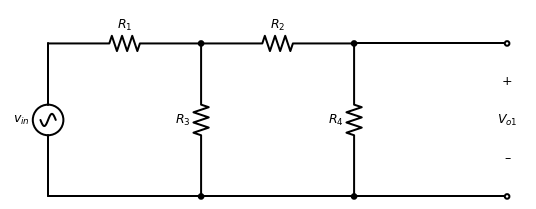
\includegraphics[scale=0.65]{p1.png}
\caption{Original circuit schematic.}
\label{fig:og_circ}
\end{figure}
%%%%%%%%%%%%%%%%%%%%%%%%%%%%%%%%%%%%%%%%%%%%

\noindent
\textbf{\emph{Find: }} The Thevenin equivalent circuit of \emph{Fig.~\ref{fig:og_circ}}.

\begin{enumerate}[label=(\alph*)]
    \item{Start by disconnecting $R_4$ (i.e. replace it with an open circuit). Find $V_{th0}$ and $R_{th0}$, the Thevenin equivalent voltage and resistance of the resulting network.}
    \item{Now, reconnect $R_4$ and find $V_{th1}$ and $R_{th1}$, the Thevenin equivalent voltage and resistance of the original network.  Express your answer in terms of $V_{th0}$ , $R_{th0}$ and $R_4$.}
    \item
        {
        Suppose we connect the following circuit to $v_{o1}$ :
        %%%%%%%%%%%%%%%%%%%%%%%%%%%%%%%%%%%%%%%%%%%%
        %                 FIGURE                   %
        %%%%%%%%%%%%%%%%%%%%%%%%%%%%%%%%%%%%%%%%%%%%
        \begin{figure}[H]
        \centering
        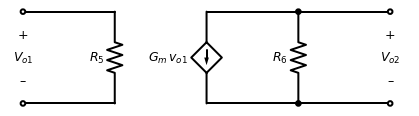
\includegraphics[scale=0.85]{p1c.png}
        \caption{Connected circuit.}
        \label{fig:add_circ}
        \end{figure}
        %%%%%%%%%%%%%%%%%%%%%%%%%%%%%%%%%%%%%%%%%%%%
        Find the output voltage $v_{o2}$ and the output resistance $R_{out}$.  Leave your answer in terms of $V_{th1}$, $R_{th1}$, $R_5$, $R_6$, and $G_m$.
        }
\end{enumerate}

\newpage\noindent
\textbf{\emph{Solution: }}

\begin{enumerate}[label=(\alph*)]
    %%%%%%%%%%%%%%%%%%
    %%% SOLUTION A %%%
    %%%%%%%%%%%%%%%%%%
    \item
        {
        By disconnecting $R_4$ from the circuit, $R_2$ is left dangling.  This means that no current can flow through it, and thus no voltage is dropped across it.  This is shown in \emph{Fig.~\ref{fig:no_r4}} below.
        %%%%%%%%%%%%%%%%%%%%%%%%%%%%%%%%%%%%%%%%%%%%
        %                 FIGURE                   %
        %%%%%%%%%%%%%%%%%%%%%%%%%%%%%%%%%%%%%%%%%%%%
        \begin{figure}[H]
        \centering
        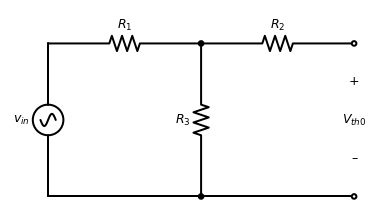
\includegraphics[scale=0.75]{p1a.png}
        \caption{The resistor $R_4$ removed leaves $R_2$ dangling.}
        \label{fig:no_r4}
        \end{figure}
        %%%%%%%%%%%%%%%%%%%%%%%%%%%%%%%%%%%%%%%%%%%%
        This results in the circuit becoming a simple voltage divider.  Then for $V_{th0}$ we have:
        
        \begin{equation*}
            \boxed{V_{th0} = v_{in} \left(\frac{R_3}{R_1 + R_3}\right)}
        \end{equation*}
        
        \vspace{0.25cm}
        Because there are no dependent sources in the circuit, the Thevenin equivalent resistance can be found by shorting out the independent voltage source, and combining the series and parallel resistances:
        
        \begin{equation*}
            \boxed{R_{th0} = R_2 + \left(R_1 \parallel R_3\right)}
        \end{equation*}
        }
    %%%%%%%%%%%%%%%%%%
    %%% SOLUTION B %%%
    %%%%%%%%%%%%%%%%%%
    \newpage\noindent
    \item
        {
        Now when we reconnect $R_4$, we can replace a portion of the circuit with the Thevenin equivalence just found in part \textit{(a)}, as shown in the \emph{Fig.~\ref{fig:r4_thev}}:
        %%%%%%%%%%%%%%%%%%%%%%%%%%%%%%%%%%%%%%%%%%%%
        %                 FIGURE                   %
        %%%%%%%%%%%%%%%%%%%%%%%%%%%%%%%%%%%%%%%%%%%%
        \begin{figure}[H]
        \centering
        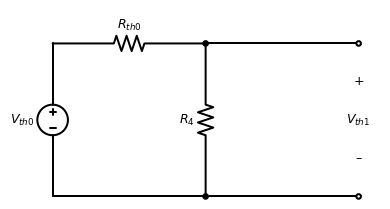
\includegraphics[scale=0.75]{p1b.png}
        \caption{$R_4$ added back in with Thevenin circuit.}
        \label{fig:r4_thev}
        \end{figure}
        %%%%%%%%%%%%%%%%%%%%%%%%%%%%%%%%%%%%%%%%%%%%
        We have another circuit that is a basic voltage divider.  First the Thevenin equivalent voltage of the original circuit:
        \begin{equation*}
            \boxed{V_{th1} = V_{th0} \left(\frac{R_4}{R_{th0} + R_4}\right)}
        \end{equation*}
        \vspace{0.25cm}
        Finally, the Thevenin equivalent resistance of the original circuit:
        
        \begin{equation*}
            \boxed{R_{th1} = R_4 \parallel R_{th0}}
        \end{equation*}
        }
    %%%%%%%%%%%%%%%%%%
    %%% SOLUTION C %%%
    %%%%%%%%%%%%%%%%%%
    \newpage\noindent
    \item
        {
        First we will start with the output voltage.  We can hook up the Thevenin equivalent circuit found in part \textit{(b)}, as shown below.
        %%%%%%%%%%%%%%%%%%%%%%%%%%%%%%%%%%%%%%%%%%%%
        %                 FIGURE                   %
        %%%%%%%%%%%%%%%%%%%%%%%%%%%%%%%%%%%%%%%%%%%%
        \begin{figure}[H]
        \centering
        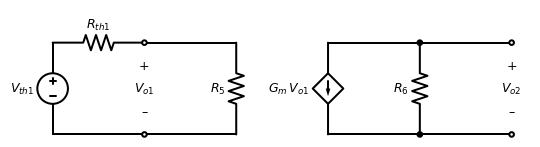
\includegraphics[scale=0.75]{p1c2.png}
        \label{fig:full_thev}
        \end{figure}
        %%%%%%%%%%%%%%%%%%%%%%%%%%%%%%%%%%%%%%%%%%%%
        Using KCL at node $V_{o2}$, and realizing that $V_{o1}$ forms a voltage divder:
        \begin{align}
            0 &= \frac{V_{o2}}{R_6} + G_m\,V_{o1}\\[0.35cm]
            &= \frac{V_{o2}}{R_6} + G_m\,V_{th1} \left(\frac{R_5}{R_5 + R_{th1}}\right)
            \label{eq:kcl}
        \end{align}
        Moving the second term in \emph{Eq.~\ref{eq:kcl}} to the other side, and multiplying both sides by $R_6$ yields the output voltage:
        \begin{equation*}
            \boxed{V_{o2} = -V_{th1}\,G_m\left(\frac{R_5\,R_6}{R_5 + R_{th1}}\right)}
        \end{equation*}
        Because we now have a dependent source, we can short the independent source and hook up a test source to $V_{o2}$ in order to find the output resistance, as shown below.
        %%%%%%%%%%%%%%%%%%%%%%%%%%%%%%%%%%%%%%%%%%%%
        %                 FIGURE                   %
        %%%%%%%%%%%%%%%%%%%%%%%%%%%%%%%%%%%%%%%%%%%%
        \begin{figure}[H]
        \centering
        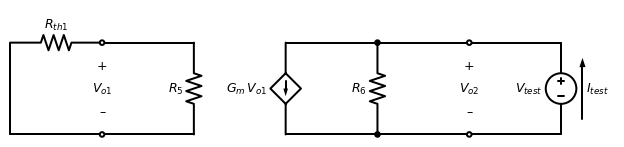
\includegraphics[scale=0.7]{p1c3.png}
        \label{fig:full_thev_test}
        \end{figure}
        %%%%%%%%%%%%%%%%%%%%%%%%%%%%%%%%%%%%%%%%%%%%
        Again, using KCL at node $V_{o2}$ gives us:
        \begin{align*}
            I_{test} &= \frac{V_{test}}{R_6} + \cancelto{0}{G_m\,V_{o1} \left(\frac{R_5}{R_5 + R_{th1}}\right)}
            &\textit{No voltage drop across $V_{o1}$}
        \end{align*}
        }
        Finally, we have the output resistance:
        \begin{equation*}
            \boxed{R_{out} = \frac{V_{test}}{I_{test}} = R_6}
        \end{equation*}
\end{enumerate}
%%%%%%%%%%%%%%%%%%%%%%%%%%%%%%%%%%%%%%%%%%%%%%%%%%%%%%%%%%%%%%%%%%%%%%%%%%%%%%%%%%%%%%%%%%%%%%%%%%%%%%%%%%%
%                                           QUESTION 2                                                    %
%%%%%%%%%%%%%%%%%%%%%%%%%%%%%%%%%%%%%%%%%%%%%%%%%%%%%%%%%%%%%%%%%%%%%%%%%%%%%%%%%%%%%%%%%%%%%%%%%%%%%%%%%%%
\newpage
\section{PN Junction Diode}
\textbf{\emph{Given: }} You are working with a foundry to design an abrupt $PN$-junction (i.e. diode), with a cross sectional area of $\num{3e-5}\,{cm}^2$, and a built-in potential of $775\,mV$ at $300^\circ K$. The donor atom concentration is set at $N_D = 10^{17}\,atoms / {cm}^3$.

\vspace{0.5cm}
\noindent
\textbf{\emph{Find: }} The following:

\begin{enumerate}[label=(\alph*)]
    \item{What is the required acceptor concentration $N_A$ in the junction?}
    \item{What is the total span of the depletion region at $1.2\,V$ reverse bias and $0\,V$ bias?}
    \item{If the foundry uses the same doping concentrations for the substrate and diffusion layers, the transistor body diodes will behave like the diodes designed above. In most circuits, these body diodes will be reverse biased and their capacitance will be a significant component in the parasitic load capacitance driven by the circuit. Assuming the same cross-sectional area from above and a bias voltage from $0\,V$ to $2.4\,V$, what is the capacitance range that you must take into consideration when designing your circuit?}
    \item{Suppose you can freely control doping concentrations ($N_D$ and $N_A$) while keeping built-in potential constant.  What is the maximum achievable junction capacitance, at $0\,V$ bias?}
\end{enumerate}

\newpage\noindent
\textbf{\emph{Solution: }}

\begin{enumerate}[label=(\alph*)]
    %%%%%%%%%%%%%%%%%%
    %%% SOLUTION A %%%
    %%%%%%%%%%%%%%%%%%
    \item
        {
        From Hu\cite{hu} (\textit{p. 93, Eq. 4.1.2}), the built-in potential is defined as:
        \begin{equation}
            \phi_{bi} = \frac{kT}{q} \cdot ln\;\bigg( \frac{N_D \cdot N_A}{{n_i}^2} \bigg)
            \label{eq:phi_bi}
        \end{equation}
        We are given $N_D$ and the built-in potential.  We also know that the thermal voltage ($\frac{kT}{q}$) at $300^\circ K$ is $\approx 0.0259\,V$, and the intrinsic concentration of $Si$ is $10^{10} / cm^3$.  Thus, rearranging \textit{Eq.~\ref{eq:phi_bi}} to solve for $N_A$:
        \begin{align*}
            N_A &= \left(\frac{{n_i}^2}{N_D}\right)
                        \cdot \mathlarger{e^{\left(\frac{\phi_{bi}}{\phi_T}\right)}}\\[0.25cm]
            &= \left(\frac{10^{20}/cm^6}{10^{17}/cm^3}\right)
                        \cdot \mathlarger{e^{\left(\frac{0.775\,V}{0.0259\,V}\right)}}\\[0.25cm]
            &= \num{9.892321044e15}/cm^3\\[0.25cm]
            \Aboxed{N_A &\approx \num{9.9e15}atoms/cm^3}
        \end{align*}
        }
    \newpage\noindent
    %%%%%%%%%%%%%%%%%%
    %%% SOLUTION B %%%
    %%%%%%%%%%%%%%%%%%
    \item
        {
        With reference to Pierret\cite{pierret} (\textit{p. 216, Eq. 5.38}), we can define the total span of the depletion region of a $PN$-junction with an applied voltage as:
        \begin{equation}
            W_{dep} = \sqrt{\frac{2\epsilon_s \left(\phi_{bi} - V_{applied}\right)}{q}
                            \cdot \Bigg( \frac{1}{N_A} + \frac{1}{N_D} \Bigg)}
            \label{eq:total_dep}
        \end{equation}        
        }
        
        Using the accepted value for the permittivity of silicon, we can plug values into \textit{Eq.~\ref{eq:total_dep}} to find the depletion region widths for the desired applied voltages.  Beginning with a $1.2\,V$ reverse bias:
        \begin{align*}
            W_{dep} &= \mathsmaller{\sqrt{\frac{2(\num{1.03545e-12}\frac{F}{cm})\left(0.775\,V - (-1.2\,V)\right)}{\num{1.602e-19}C}
                            \cdot \Bigg( \frac{1}{\num{9.9e15}/cm^3} + \frac{1}{10^{17}/cm^3} \Bigg)}}\\[0.25cm]
            &= \sqrt{\frac{\num{2.0709e-12}\frac{\cancel{A \cdot s}/\bcancel{V}}{cm}\left(1.975\,\bcancel{V}\right)}{\num{1.602e-19}\cancel{A \cdot s}}
                            \cdot \Big(\num{1.111e-16}\,cm^3\Big)}\\[0.25cm]
            &= \sqrt{\frac{25527943.98}{\cancel{cm}} \cdot \Big(\num{1.111e-16}\,cm^{\cancelto{2}{3}}\Big)}\\[0.25cm]
            &= \sqrt{\num{2.836154576e-9}\,{cm}^2}\\[0.25cm]
            &= \num{5.325555911e-5}\,cm\\[0.25cm]
            \Aboxed{W_{dep} &\approx 0.533\,\mu m}
        \end{align*}

        Now for no applied bias ($0\,V$), for which we expect a smaller depletion region:
        \begin{align*}
            W_{dep} &= \sqrt{\frac{(\num{2.0709e-12}/cm) \cdot (0.775\,V)}{\num{1.602e-19}}
                            \cdot \Big(\num{1.111e-16}\,cm^3\Big)}\\[0.25cm]
            &= \sqrt{\frac{10017294.47}{\cancel{cm}} \cdot \Big(\num{1.111e-16}\,cm^{\cancelto{2}{3}}\Big)}\\[0.25cm]
            &= \sqrt{\num{1.112921416e-9}\,{cm}^2}\\[0.25cm]
            &= \num{3.336047686e-5}\,cm\\[0.25cm]
            \Aboxed{W_{dep} &\approx 0.334\,\mu m}
        \end{align*}

    \newpage\noindent
    %%%%%%%%%%%%%%%%%%
    %%% SOLUTION C %%%
    %%%%%%%%%%%%%%%%%%
    \item
        {
        With reference to Hu\cite{hu} (\textit{p. 98, Eq. 4.41}), the depletion capacitance of a $PN$-junction is defined as:
        \begin{equation}
            C_{dep} = A \left(\frac{\epsilon_s}{W_{dep}}\right)
            \label{eq:junc_cap}
        \end{equation}
        }
        
        We know the cross-sectional area, and already found the depletion region width for $0\,V$ in part (b).  So we can use that result to find one bound:
        \begin{align*}
            C_{dep} &= \num{3e-5}\,{cm}^2 \left(\frac{\num{1.03545e-12}\frac{F}{cm}}{\num{3.336047686e-5}\,cm}\right)\\[0.25cm]
            &= \num{3e-5}\,\cancel{{cm}^2} \left(\num{3.103822539e-8}\frac{F}{\cancel{{cm}^2}}\right)\\[0.25cm]
            &= \num{9.31146762e-13}\,F\\[0.25cm]
            \Aboxed{&\approx 0.931\,pF}
        \end{align*}
        
        Next, we will find the depletion region for a $2.4\,V$ reverse bias:
        \begin{align*}
            W_{dep} &= \mathsmaller{\sqrt{\frac{2(\num{1.03545e-12}\frac{F}{cm})\left(0.775\,V - (-2.4\,V)\right)}{\num{1.602e-19}C}
                            \cdot \Bigg( \frac{1}{\num{9.9e15}/cm^3} + \frac{1}{10^{17}/cm^3} \Bigg)}}\\[0.25cm]
            &= \sqrt{\frac{\num{2.0709e-12}\frac{\cancel{A \cdot s}/\bcancel{V}}{cm}\left(3.175\,\bcancel{V}\right)}{\num{1.602e-19}\cancel{A \cdot s}}
                            \cdot \Big(\num{1.111e-16}\,cm^3\Big)}\\[0.25cm]
            &= \sqrt{\frac{41038593.49}{\cancel{cm}} \cdot \Big(\num{1.111e-16}\,cm^{\cancelto{2}{3}}\Big)}\\[0.25cm]
            &= \sqrt{\num{4.559387736e-9}\,{cm}^2}\\[0.25cm]
            &= \num{6.752323849e-5}\,cm
        \end{align*}

        Then we can use this result to find the other bound:
        \begin{align*}
            C_{dep} &= \num{3e-5}\,{cm}^2 \left(\frac{\num{1.03545e-12}\frac{F}{cm}}{\num{6.752323849e-5}\,cm}\right)\\[0.25cm]
            &= \num{3e-5}\,\cancel{{cm}^2} \left(\num{1.533472066e-8}\frac{F}{\cancel{{cm}^2}}\right)\\[0.25cm]
            &= \num{4.6004162e-13}\,F\\[0.25cm]
            \Aboxed{&\approx 0.46\,pF}
        \end{align*}
        
        Thus, we should be concerned with the capacitance range of: $\boxed{\big[0.46\,pF,\;0.931\,pF\big]}$
    \newpage\noindent
    %%%%%%%%%%%%%%%%%%
    %%% SOLUTION D %%%
    %%%%%%%%%%%%%%%%%%
    \item
        {
        From \textit{Eq.~\ref{eq:total_dep}} we can see that larger doping concentrations result in a smaller total depletion region.  Additionally, from \textit{Eq.~\ref{eq:junc_cap}} we know that a smaller depletion region results in a larger junction capacitance.  Thus, for the maximum achievable junction capacitance we want the largest possible doping concentration.
        
        However, from \textit{Eq.~\ref{eq:phi_bi}} we can also see that the factor $N_A \cdot N_D$ must also remain constant for the built-in potential to remain constant.  This means the if we raise one doping, then we must lower the other proportionally.  Thus, this becomes a minimization problem, one in which we will use calculus to solve.  We want to minimize the doping term in the depletion region equation, which we can rewrite:
        \begin{equation}
            \frac{1}{N_A} + \frac{1}{N_D} = \frac{N_A + N_D}{N_A\,N_D}
            \label{eq:dope_par}
        \end{equation}
        
        Specifically, we want to minimize the numerator of the term on the RHS of \textit{Eq.~\ref{eq:dope_par}}.  So we let $k = N_A \cdot N_D$ and substitute for $N_D$, and define the function we want to minimize:
        \begin{equation}
            \beta (N_A) = N_A + \frac{k}{N_A}
            \label{eq:dope_min}
        \end{equation}
        Now differentiating \textit{Eq.~\ref{eq:dope_min}}, and setting equal to zero in order to find the local minima:
        \begin{align*}
            \beta '(N_A) &= \frac{d}{d\,N_A}\left(N_A + \frac{k}{N_A}\right)\\[0.25cm]
            &= 1 + k \cdot \left(\frac{-1}{{N_A}^2}\right) = 0
        \end{align*}
        
        Rearranging and solving for $N_A$ gives us:
        \begin{equation}
            N_A = \sqrt{k} = \sqrt{N_A \cdot N_D}
            \label{eq:new_na}
        \end{equation}

        Plugging in our known dopings that yield $775\,mV$ from earlier gives us the doping we want to use for the new $N_A$:
        \begin{align*}
            N_{A_{new}} &= \sqrt{\num{9.9e15}/cm^3 \cdot \num{1e17}/cm^3}\\[0.25cm]
            &= \num{3.146426545e16}/cm^3\\[0.25cm]
            \Aboxed{&\approx \num{3.15e16}/cm^3}
        \end{align*}

        Now for the new $N_D$:
        \begin{align*}
            N_{D_{new}} &= \frac{k}{N_{A_{new}}}\\[0.25cm]
            &= \frac{\num{9.9e15}/cm^3 \cdot \num{1e17}/cm^3}{\num{3.146426545e16}/cm^3}\\[0.25cm]
            &= \num{3.146426545e16}/cm^3\\[0.25cm]
            \Aboxed{&\approx \num{3.15e16}/cm^3}
        \end{align*}

        \vspace{0.15cm}
        We have a new and equal doping concentration for both sides of the junction.  Now we can figure out the new depletion width:
        \begin{align*}
            W_{dep} &= \sqrt{\frac{2\epsilon_s\,\phi_{bi}}{q} \cdot \Bigg( \frac{1}{N_A} + \frac{1}{N_D} \Bigg)}\\[0.25cm]
            &= \sqrt{\frac{2(\num{1.03545e-12}\frac{F}{cm})(0.775\,V)}{\num{1.602e-19}C}
                    \cdot \Bigg( \frac{1}{\num{3.15e16}/cm^3} + \frac{1}{\num{3.15e16}/cm^3} \Bigg)}\\[0.25cm]
            &= \sqrt{\frac{10017294.47}{cm} \cdot \left(\num{6.35641726e-17}cm^3\right)}\\[0.25cm]
            &= \sqrt{\num{6.35641726e-10}\,cm^2}\\[0.25cm]
            &= \num{2.523372812e-5}\,cm
        \end{align*}        
        }
        
        Thus, the maximum achievable junction capacitance, given a $0\,V$ bias and fixed $\phi_{bi}$: 
        \begin{align*}
            C_{dep} &= \num{3e-5}\,{cm}^2 \left(\frac{\num{1.03545e-12}\frac{F}{cm}}{\num{2.523372812e-5}\,cm}\right)\\[0.25cm]
            &= \num{3e-5}\,\cancel{{cm}^2} \left(\num{4.10343646e-8}\frac{F}{\cancel{{cm}^2}}\right)\\[0.25cm]
            &= \num{1.23103094e-12}\,F\\[0.25cm]
            \Aboxed{&\approx 1.23\,pF}
        \end{align*}

\end{enumerate}
%%%%%%%%%%%%%%%%%%%%%%%%%%%%%%%%%%%%%%%%%%%%%%%%%%%%%%%%%%%%%%%%%%%%%%%%%%%%%%%%%%%%%%%%%%%%%%%%%%%%%%%%%%%
%                                           QUESTION 3                                                    %
%%%%%%%%%%%%%%%%%%%%%%%%%%%%%%%%%%%%%%%%%%%%%%%%%%%%%%%%%%%%%%%%%%%%%%%%%%%%%%%%%%%%%%%%%%%%%%%%%%%%%%%%%%%
\newpage
\section{MOS Transistor IV Curve}
\textbf{\emph{Given: }} A long channel $5V\;PMOS$ transistor has been characterized with the following parameters:
    \begin{table}[H]
    \centering
    \setlength{\tabcolsep}{20pt}
    \renewcommand{\arraystretch}{1.5}
        \begin{tabular}{|l|c|}
            \hline
            $W$ & $10\,\mu m$\\
            \hline
            $L$ & $1\,\mu m$\\
            \hline
            $\mu C_{ox}$ & $-100\,\mu A/V^2$\\
            \hline
            $\lambda$ & $0.024\,V^{-1}$\\
            \hline
            $V_{th}$ & $-0.6\,V$\\
            \hline
        \end{tabular}
    \label{tab:pmos}
    \end{table}

\noindent
\textbf{\emph{Find: }} The following:

\begin{enumerate}[label=(\alph*)]
    \item{Sketch, by hand or with MATLAB, the device current $I_D$ vs. $V_{GS}$ from $-0.6\,V$ to $-5\,V$ for $V_{DS}$ equal to $-1.5\,V$ and $-4.5\,V$. Explain the difference in the shape of the curves for the different $V_{DS}$.  Assume $V_{SB} = 0$.}
    \item{Sketch, by hand or with MATLAB, the device current $I_D$ vs. $V_{DS}$ from $0\,V$ to $-5\,V$ for $V_{GS}$ equal to $0.8\,V$, $-1.6\,V$ and $-3.2\,V$. Assume $V_{SB} = 0$.  Clearly label each region of operation.}
    \item{Explain how the plot in \textit{(a)} and \textit{(b)} would change if this was a short-channel device.}
\end{enumerate}

\newpage\noindent
\textbf{\emph{Solution:}}
        The plots were constructed in MATLAB using a piece-wise defined function based on the following definitions.
        In the table below are the conditions for each region of operation of an $NMOS$ and $PMOS$.  We will flip the polarities of the given values for the $PMOS$ in order to make the plots look similar to an $NMOS$.
        \begin{table}[H]
        \centering
        \setlength{\tabcolsep}{20pt}
        \renewcommand{\arraystretch}{1.5}
        \begin{tabular}{|l|c|c|c|}
            \hline
            \textbf{Transistor Type}  &  \textbf{Cut-off} & \textbf{Triode} & \textbf{Saturation}\\
            \hline
            \textit{NMOS} & $V_{GS} \leq V_{T_n}$
                            & $V_{DS} \leq V_{GS} - V_{T_n}$
                            & $V_{DS} > V_{GS} - V_{T_n}$\\
            \hline
            \textit{PMOS} & $V_{SG} \leq \left|V_{T_p}\right|$
                            & $V_{SD} \leq V_{SG} - \left|V_{T_p}\right|$
                            & $V_{SD} > V_{SG} - \left|V_{T_p}\right|$\\
            \hline
        \end{tabular}
        \caption{Conditions for MOSFET regions of operation.
        \label{tab:imp}} 
        \end{table}
        With reference to Razavi\cite{raz} (\textit{pp. 14-15}), we can define the current of a $PMOS$ for the triode and saturation regions as follows:
        \begin{align}
           I_{SD,sat} &= \left(\frac{W}{2L}\right) \mu_p\,C_{ox}
                             {\big(V_{SG} - \left|V_{T_p}\right|\big)}^2 (1 + \lambda V_{SD})
            &\textit{$PMOS$ saturation current}
            \label{eq:mosfet_ids_pmos}\\[0.25cm]
            I_{SD,tri} &= \left(\frac{W}{L}\right) \mu_p\,C_{ox} \left(V_{SG} - \left|V_{T_p}\right| - \frac{V_{SD}}{2}\right) V_{SD}
            &\textit{$PMOS$ triode current}
            \label{eq:mosfet_ids_pmos_tri}
        \end{align}

\begin{enumerate}[label=(\alph*)]
    %%%%%%%%%%%%%%%%%%
    %%% SOLUTION A %%%
    %%%%%%%%%%%%%%%%%%
    \item
        {
        Below is a plot of both curves for the different values of $V_{SD}$.  When $V_{SD}= 4.5\,V$, the device is immediately placed in saturation once the gate voltage moves beyond threshold, and the curve is only quadratic.  At $V_{SD} = 1.5\,V$, the device can operate in the triode region, and we see a linear portion in the curve.
        %%%%%%%%%%%%%%%%%%%%%%%%%%%%%%%%%%%%%%%%%%%
        %                 FIGURE                   %
        %%%%%%%%%%%%%%%%%%%%%%%%%%%%%%%%%%%%%%%%%%%%
        \begin{figure}[H]
        \centering
        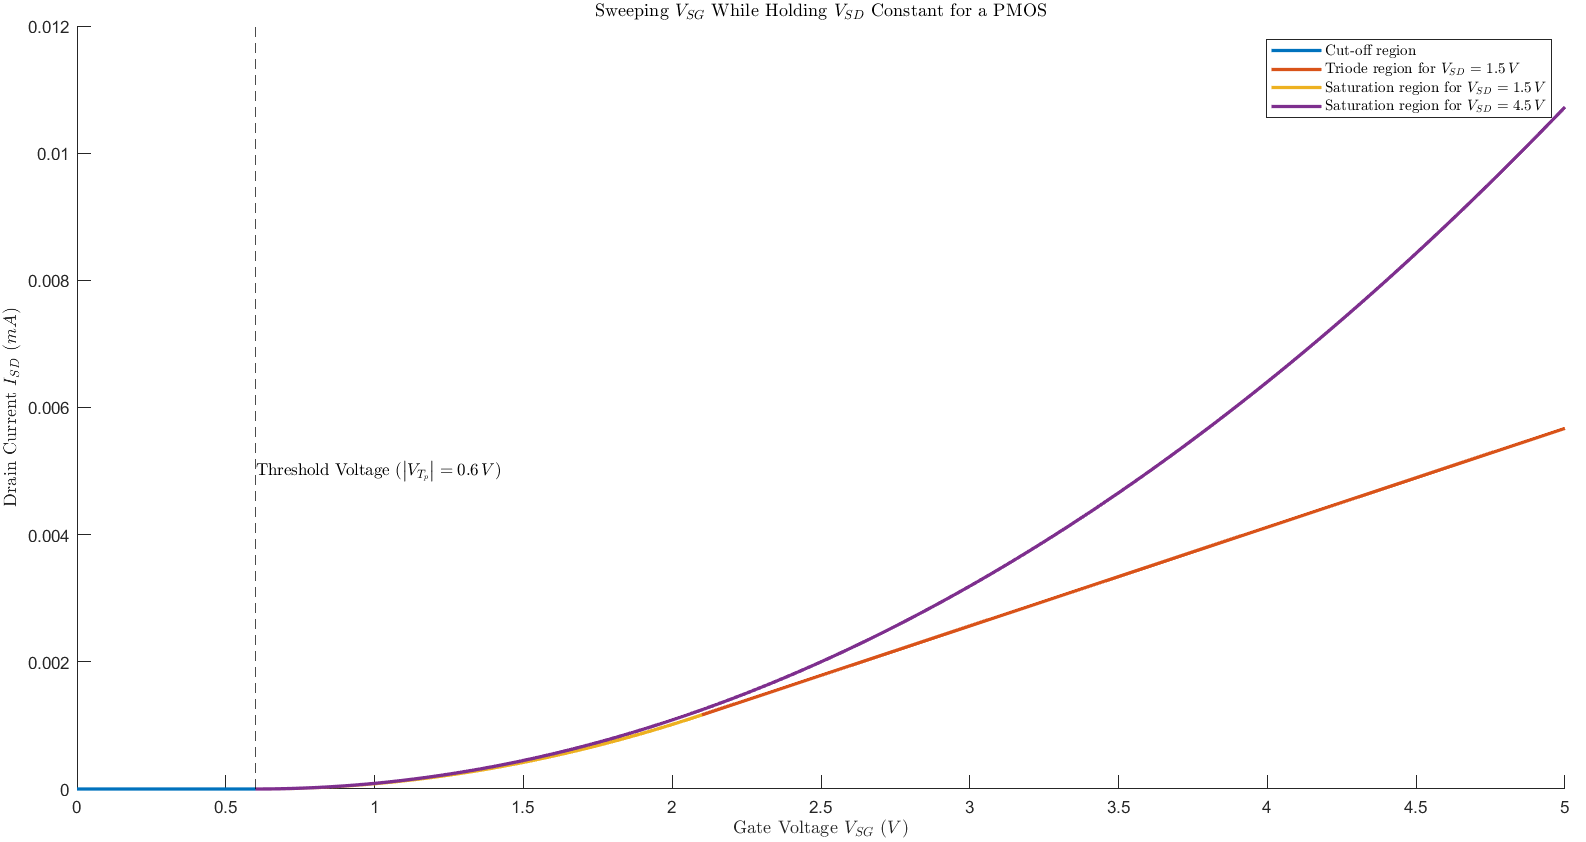
\includegraphics[scale=0.4]{p3a.png}
        \label{fig:input_char}
        \end{figure}
        %%%%%%%%%%%%%%%%%%%%%%%%%%%%%%%%%%%%%%%%%%%%
        }

    \newpage\noindent
    %%%%%%%%%%%%%%%%%%
    %%% SOLUTION B %%%
    %%%%%%%%%%%%%%%%%%
    \item
        {
        Below is a plot of both curves for the different values of $V_{SG}$.  When $V_{SG}= -0.8\,V$, the device is in cut-off, and it will never turn on.  The larger overdrive voltage results in a larger transconductance amplifier, which is why the drain current in saturation is larger for the larger gate voltage.
        %%%%%%%%%%%%%%%%%%%%%%%%%%%%%%%%%%%%%%%%%%%%
        %                 FIGURE                   %
        %%%%%%%%%%%%%%%%%%%%%%%%%%%%%%%%%%%%%%%%%%%%
        \begin{figure}[H]
        \centering
        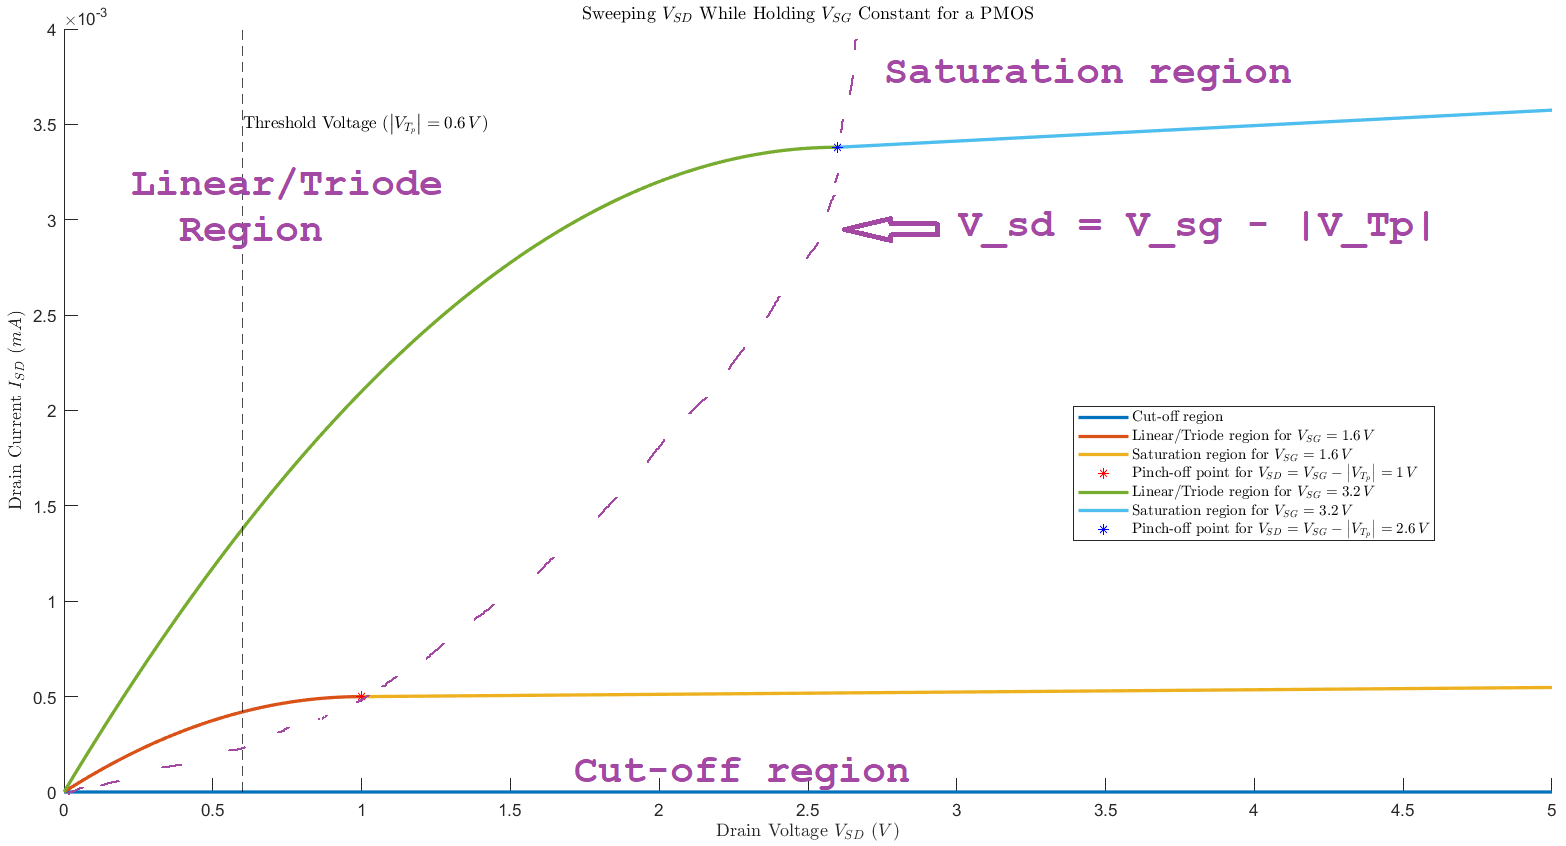
\includegraphics[scale=0.4]{p3b.png}
        \label{fig:output_char}
        \end{figure}
        %%%%%%%%%%%%%%%%%%%%%%%%%%%%%%%%%%%%%%%%%%%%
        }

    %%%%%%%%%%%%%%%%%%
    %%% SOLUTION C %%%
    %%%%%%%%%%%%%%%%%%
    \item
        {
        In a short-channel device, the electric field will be much stronger because of the decreased channel length.  This will cause the carriers to reach a saturation velocity sooner than they would in a long-channel device.  Because of this the current is decreased, and the device will behave linearly.  This means that the plot in \textit{(a)} will only have a linear region, and the plot in \textit{(b)} will have a larger slope in saturation due to the increased channel length modulation.
        }
\end{enumerate}
%%%%%%%%%%%%%%%%%%%%%%%%%%%%%%%%%%%%%%%%%%%%%%%%%%%%%%%%%%%%%%%%%%%%%%%%%%%%%%%%%%%%%%%%%%%%%%%%%%%%%%%%%%%
%                                           BIBLIOGRAPHY                                                  %
%%%%%%%%%%%%%%%%%%%%%%%%%%%%%%%%%%%%%%%%%%%%%%%%%%%%%%%%%%%%%%%%%%%%%%%%%%%%%%%%%%%%%%%%%%%%%%%%%%%%%%%%%%%
\newpage
\addcontentsline{toc}{section}{References}
\emergencystretch=2em
\nocite{*}
\printbibliography
%%%%%%%%%%%%%%%%%%%%%%%%%%%%%%%%%%%%%%%%%%%%%%%%%%%%%%%%%%%%%%%%%%%%%%%%%%%%%%%%%%%%%%%%%%%%%%%%%%%%%%%%%%%
%                                           END OF DOCUMENT                                               %
%%%%%%%%%%%%%%%%%%%%%%%%%%%%%%%%%%%%%%%%%%%%%%%%%%%%%%%%%%%%%%%%%%%%%%%%%%%%%%%%%%%%%%%%%%%%%%%%%%%%%%%%%%%
\end{document}
